% gEDA - GPL Electronic Design Automation
% cascade.tex - RF Cascade symbol library and gnetlist backend documentation
% Copyright (C) 2003 Dan McMahill
%
% This program is free software; you can redistribute it and/or modify
% it under the terms of the GNU General Public License as published by
% the Free Software Foundation; either version 2 of the License, or
% (at your option) any later version.
%
% This program is distributed in the hope that it will be useful,
% but WITHOUT ANY WARRANTY; without even the implied warranty of
% MERCHANTABILITY or FITNESS FOR A PARTICULAR PURPOSE.  See the
% GNU General Public License for more details.
%
% You should have received a copy of the GNU General Public License
% along with this program; if not, write to the Free Software
% Foundation, Inc., 675 Mass Ave, Cambridge, MA 02139, USA.

\documentclass{article}
\usepackage{graphicx}
% This line will enable hyperlinks in the PDF output
% file.
\usepackage[ps2pdf,breaklinks=true,colorlinks=true]{hyperref}

\setlength{\parindent}{0pt}
\setlength{\parskip}{1ex plus 0.5ex minus 0.2ex}

\title{gEDA/gaf RF Cascade  Symbols and Netlister}
\author{Dan McMahill\\
        \\
        This document is released under GFDL\\ 
        (\url{http://www.gnu.org/copyleft/fdl.html})}
\date{December 3rd, 2003}

\begin{document}

\maketitle
\newpage

\tableofcontents
\newpage


\section{Overview}
This document describes the symbol library and gnetlist backend which
support driving RF Cascade (\url{http://rfcascade.sourceforge.net})
simulations from the gEDA/gaf system.
Cascade is a noise figure and distortion analysis tool geared towards
radio receiver design.

The basic steps involved with using gEDA as the frontend for Cascade
simulations are:

\begin{enumerate}
\item Create schematics of the circuit.
\item Extract the netlist.
\item Run Cascade.
\end{enumerate}

\section{Requirements}
You will need the following programs to be installed.
\begin{enumerate}
\item A recent version of gEDA/gaf.  To see if your version is recent
  enough, see if the directory {\tt \${prefix}/share/gEDA/sym/cascade}
  exists.  {\tt \${prefix}} is the installation prefix for gEDA on
  your system.

\item RF Cascade.  The executable is usually called {\tt cascade}.  
  If you do
  not have Cascade available on your system, you will need to get a copy
  from \url{http://rfcascade.sourceforge.net}.
\end{enumerate}

\section{Creating Schematics}
When creating a block diagram in the {\tt gschem} schematic editor,
use only the symbols from the cascade library.  Every block diagram
must have a ``cascade-source'' element.  In addition, the block
diagram must be a simple cascade.  No parallel paths or branches are
allowed.

All instances must have a unique reference designator.  For a receiver
block diagram, this is often times best achieved by manually entering
them.  The only restriction on reference designator names is that they
contain no spaces.  A descriptive name such as ``RF\_Filter'' or
``First\_Mixer'' is useful as it will show up in the cascade output
report. 

\section{Extracting the Cascade Input File}
To extract the Cascade input file, run
\begin{verbatim}
    gnetlist -g cascade -o test.cas file1.sch [file2.sch ...]
\end{verbatim}
For the example file contained in this archive, you can run: 
\begin{verbatim}
    gnetlist -g cascade -o example.cas example.sch
\end{verbatim}

The netlist will be left in {\tt example.cas}.

\section{Running Cascade}
Cascade is exceptionally simple to run.  Just run
\begin{verbatim}
    cascade example.cas > example.out
\end{verbatim}
to run the analysis on the system contained in the file
{\tt example.cas} and write the results to the file
{\tt example.out}.  Refer to the Cascade documentation 
for complete details.

\appendix
\section{Symbols in the Library}
Please note that all instances must have  the
{\tt refdes=} attribute set.

\subsection{Sources (cascade-source)}
Source. \\
Attributes:
\begin{itemize}
\item {\bf C}=Carrier level in dBm.  Optional.
\item {\bf CN0}=Carrier to Noise Spectral Density Ratio in dBm/Hz.  Optional.
\item {\bf CN}=Carrier to Noise Ratio in dB.  Optional.
\item {\bf BW}=Signal Bandwidth in Hz.  Optional, but requred if {\tt
    CN=} is used.
\end{itemize}

\subsection{Defaults (cascade-default)}
This symbol sets the default impedance levels as well as the
correlation coefficient used for third order distortion calculations.
There are two versions of this symbol.  One is used to set the
defaults at the beginnng of the definition.  The other can be placed
in series with the cascade to change the defaults part way through.
This is useful if you wish to change impedance levels in the middle of
the receiver chain. \\
Attributes:
\begin{itemize}
\item {\bf RIN}=Default block input resistance in Ohms.  Optional.
\item {\bf ROUT}=Default block output resistance in Ohms.  Optional.
\item {\bf RHO}=Default third order distortion correlation
  coefficient.  Optional.
\end{itemize}

\subsection{Elements}
Cascade characterizes each block in a system by its gain and optionally
noise figure and third order intercept point.  As such, there is
no distinction between various elements such as amplifiers, filters, and
mixers.  The gEDA/gaf RF Cascade symbol library contains different
symbols for clarity in the diagram only.  The currently available
element symbols are:
\begin{table}[h]
\begin{center}
\begin{tabular}{||l|l||} \hline \hline
cascade-amp           & Amplifier    \\ \hline 
cascade-filter        & Filter       \\ \hline 
cascade-mixer         & Mixer        \\ \hline 
cascade-transformer   & Transformer  \\ \hline 
\hline
\end{tabular}
\caption{Element Types}
\label{tab:elements}
\end{center}
\end{table}
Attributes:
\begin{itemize}
\item Gain is specified by one of the following:
  \begin {itemize}
  \item {\bf G}=Power gain in dB.
  \item {\bf GP}=Power gain in dB.
  \item {\bf GV}=Voltage gain in dB.
  \end {itemize}
\item {\bf NF}=Noise Figure in dB.  Optional.
\item {\bf IIP3}=Input Third Order Intercept Point in dBm.  Optional.
\item {\bf RIN}=Block input resistance in Ohms.  Optional.
\item {\bf ROUT}=Block output resistance in Ohms.  Optional.
\item {\bf RHO}=Third order distortion correlation coefficient.  Optional.
\end{itemize}
\section{Example}
This appendix provides a simple example of the entire process of
generating a schematic, producing a Cascade input file,
running an analysis and looking at the result.

\subsection{Example Schematics}
Figure~\ref{fig:ckt} shows the
schematic of a simple receiver signal chain.
\begin{figure}
\begin{center}
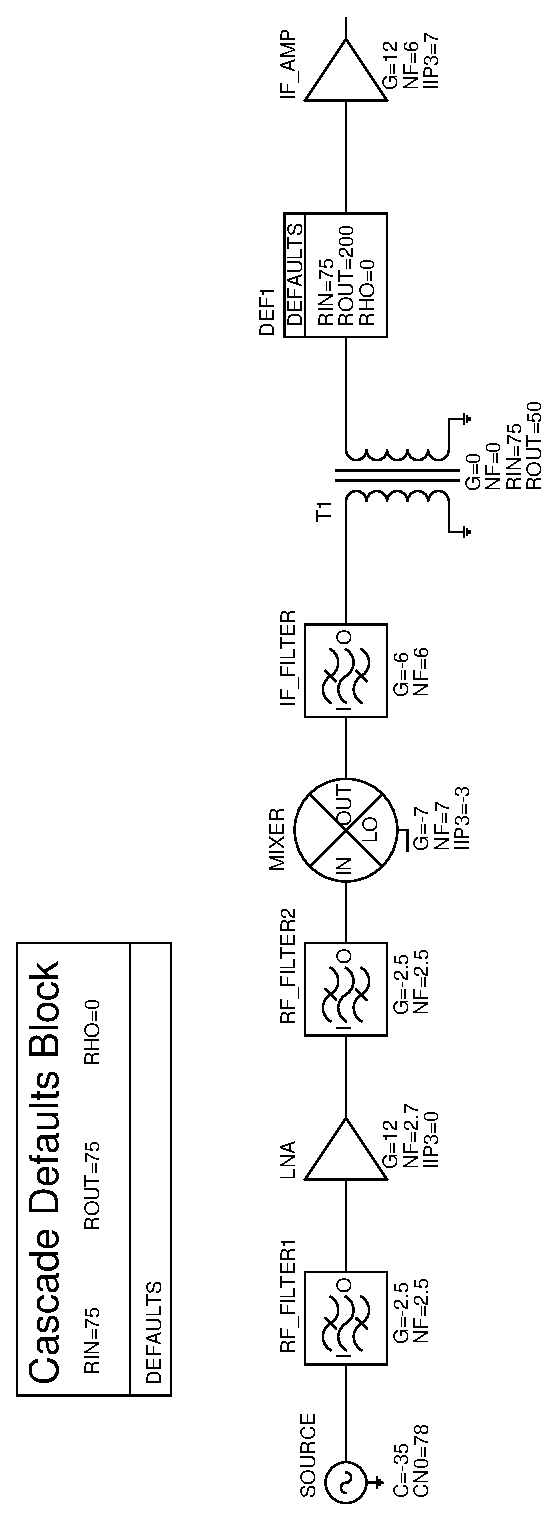
\includegraphics[angle=270,width=4in]{example.eps}
\end{center}
\caption{Simple Receiver Signal Chain Block Diagram}
\label{fig:ckt}
\end{figure}
Figure~\ref{fig:example.cas} shows
the contents of the {\tt example.cas} file.
\begin{figure}
\begin{verbatim}

# Cascade (http://rfcascade.sourceforge.net)
# Created with gEDA/gnetlist

# Initial global defaults
defaults RIN=75 ROUT=75 RHO=0 

source C=-35 CN0=78 
RF_FILTER1 G=-2.5 NF=2.5 
LNA G=12 NF=2.7 IIP3=0 
RF_FILTER2 G=-2.5 NF=2.5 
MIXER G=-7 NF=7 IIP3=-3 
IF_FILTER G=-6 NF=6 
T1 G=0 NF=0 RIN=75 ROUT=50 
defaults RIN=75 ROUT=200 RHO=0 
IF_AMP G=12 NF=6 IIP3=7 

# End of netlist created by gEDA/gnetlist

\end{verbatim}
\caption{Example RF Cascade Input File, {\tt example.cas}}
\label{fig:example.cas}
\end{figure}

\subsection{Netlist the Design}
To netlist the design, run:
\begin{verbatim}
    gnetlist -g cascade example.cas example.sch
\end{verbatim}

\subsection{Run the Analysis}
Run the analysis with:
\begin{verbatim}
    cascade example.cas
\end{verbatim}
\newpage
\section{Document Revision History}

\begin{table}[h]
\begin{tabular}{|l|l|} \hline
December 3rd, 2003 & Created cascade.tex \\ \hline
\end{tabular}
\end{table}

\end{document}

